%!TEX root=ClassNotes.tex
\section{Fundamental Theorem of Calculus}

The Fundamental Theorem of Calculus is a remarkable theorem that connects the notions of derivatives and integrals.

If we denote by $\mathcal{D}$ the {\it operator} that takes a function and produces it's derivative i.e. $\mathcal{D}(f) = f'$ and by $\mathcal{I}$ the {\it operator} that takes a function and produces (one of) it's antiderivative i.e. $\mathcal{I}(f) = \int_a^x f(t) \: \:dt$, for some real number $a$, then the Fundamental Theorem of Calculus says that
\begin{enumerate}
	\item $\mathcal{D}(\mathcal{I}(f)) = f$, and
	\item  $\mathcal{I}(\mathcal{D}(f)) = f + $ a constant.
\end{enumerate} so that Integral and Derivative are (almost) inverse operators.\footnote{Compare this to the definition of inverse functions: $f(g(x)) = x$ and $g(f(x)) = x$.} This is why $\int_a^x f(t) \: \:dt$ is called (an) {antiderivative}.\\



\begin{theorem}[Fundamental Theorem of Calculus]$ $
	\begin{description}
		\item[Form 1] Let $f$ be a continuous function. For a real number $a$, let $ F_a(x) = \int \limits_a^x f(t) \:dt$.
		      Then $F_a(x)$ is differentiable with
		      \begin{align*}
			      F_a'(x) = f(x).
		      \end{align*}
		\item[Form 2]
		      Let $f$ be a differentiable function with $f'$ continuous. Then for any real numbers $a$ and $x$,
		      \begin{align*}
			      \int \limits_a^x f'(t) \:dt = f(x) - f(a).
		      \end{align*}
	\end{description}
\end{theorem}

The idea of the proof of Form 1 is very straightforward. By definition of derivative,
\begin{align}
	\begin{split}
		F_a'(x)
		& = \lim \limits_{h \rightarrow 0} \dfrac{F_a(x+h) - F_a(x)}{h}                                                                                                 \\
		& = \lim \limits_{h \rightarrow 0} \dfrac{\int \limits_a^{x+h} f(t) \:dt - \int \limits_a^x f(t) \:dt}{h}                                                           \\
		& = \lim \limits_{h \rightarrow 0} \dfrac{\int \limits_x^{x+h} f(t) \:dt}{h}
		\qquad
		\qquad
		\mbox{ by Exercise } \ref{q:difference_antiderivatives}
	\end{split}
	\label{eq:Fundamental_Theorem_Reduction}
\end{align}
For small $h$ this last integral can be approximated by the area of a rectangle with height $f(x)$ and base $h$.
\begin{align*}
	\int \limits_x^{x+h} f(t) \:dt
	 & \approx f(x) \cdot h \\
	\implies \dfrac{\int \limits_x^{x+h} f(t) \:dt}{h}
	 & \approx f(x)
\end{align*}
We'll make this last statement precise using $\epsilon, \delta$ arguments. We'll start with a small Proposition.
\begin{figure}[t]
	\centering
	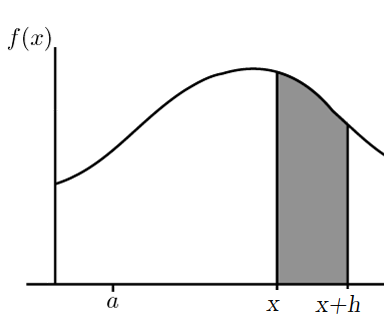
\includegraphics[width=0.6\textwidth]{FundamentalTheorem.png}
	\caption*{The area $\int_x^{x+h} f(t)\:dt$ can be approximated by a rectangle with height $f(x)$ and base $h$.}
\end{figure}

\begin{prop}
	\label{theorem:Fundamental_theorem_lemma}
	If for all $ y$ in the interval $(x,x+h)$,
	\begin{align*}
	m < f(y) < M
	\end{align*}
	for some real numbers $m$, $M$, then
	\begin{align*}
		mh < \int \limits_{a}^{b} f(t) \: \:dt < Mh
	\end{align*}
\end{prop}
\begin{exercise}$ $
	\begin{enumerate}
		\item Prove the above Proposition using a {\it geometric} argument.
		\item \textbf{Optional: } Prove the above Proposition rigorously using the definition of integral involving Riemann sums.
	\end{enumerate}
\end{exercise}

Now we get back to the proof of the Form 1 of the Fundamental Theorem of Calculus.
\begin{proof}[Proof of Form 1 of the Fundamental Theorem of Calculus]
	Let $f(x)$ be a continuous function, let $a$ be a real number. We want to show that
	\begin{align*}
		F_a'(x) = f(x)
	\end{align*}
	By Equations \eqref{eq:Fundamental_Theorem_Reduction} this is equivalent to proving that
	\begin{align*}
		\lim \limits_{h \rightarrow 0}\dfrac{\int \limits_x^{x+h} f(t) \:dt}{h}
		 & = f(x)
	\end{align*}
	We'll only prove this for the right hand limit, the left hand limit is proved similarly. We want to show that
	\begin{align}
		\label{eq:Fundamental_theorem_limit}
		\lim \limits_{h \rightarrow 0^+}\dfrac{\int \limits_x^{x+h} f(t) \:dt}{h}
		 & = f(x)
	\end{align}
	\begin{exercise}
		\label{q:epsilon_delta_limit}
		Convert Equation \eqref{eq:Fundamental_theorem_limit} into an $\epsilon, \delta$ statement using the definition of limit.
	\end{exercise}

	\begin{exercise}
		Recall what it means for $f(x)$ to be continuous from the right, using the  $\epsilon, \delta$ definition of continuity.
	\end{exercise}

	\begin{exercise}
		Using this $\delta$ and Proposition \ref{theorem:Fundamental_theorem_lemma} prove the statement in Exercise \ref{q:epsilon_delta_limit}, thereby completing the proof of the Fundamental Theorem of Calculus.
	\end{exercise}
\end{proof}

\begin{exercise}[{\bf Optional}]
	Prove that $\lim \limits_{h \rightarrow 0^-}\dfrac{\int \limits_x^{x+h} f(t) \:dt}{h}
	= f(x)$. (Be careful of the signs.)
\end{exercise}


The Form 2 of the fundamental theorem follows directly from Form 1 using a small Proposition about derivatives.
\begin{prop}
	\label{theorem:Fundamental_theorem_lemma2}
	If $g(x)$ is a differentiable function such that $g'(x) = 0$ for all real numbers $x$, then $g(x)$ is a constant function i.e. $g(x) = g(y)$ for all real numbers $x$, $y$.
\end{prop}
\begin{exercise}
	Prove the above Proposition by Contradiction\hint{Use the Mean Value Theorem}.
\end{exercise}

\begin{proof}[Proof of Form 2 of the Fundamental Theorem of Calculus]
	Let $f$ be a diffentiable function with $f'$ continuous, and let $a$ be a real number. We want to show that
	\begin{align*}
		\int \limits_a^x f'(t) \:dt = f(x) - f(a)
	\end{align*}
	Consider the function
	\begin{align*}
		g(x) = f(x) - \int \limits_a^x f'(t) \:dt.
	\end{align*}
	\begin{exercise}
		Using Form 1 of the Fundamental Theorem and Proposition \ref{theorem:Fundamental_theorem_lemma2} prove that $g(x)$ is a constant function.
	\end{exercise}
	\begin{exercise}
		As $g$ is a constant function, for all real numbers $x$, $g(x) = g(a)$. Use this to prove Form 2 of the Fundamental Theorem of Calculus.
	\end{exercise}
\end{proof}

\begin{remark}
	For real numbers $b$, $c$,
		\begin{align*}
			\int \limits_b^c f(t) \:dt
			&= \int \limits_b^a f(t) \:dt + \int \limits_a^c f(t) \:dt\\
			&= -\int \limits_a^b f(t) \:dt + \int \limits_a^c f(t) \:dt\\
			&= F_a(c) - F_a(b)
		\end{align*}
	where $F_a(x)$ is {\it an} antiderivative of $f(x)$ i.e. it is a function whose derivative is $f(x)$. This is the form is which the Fundamental Theorem of Calculus is most often used. Which $a$ we use to find the antiderivative does not matter, so the integral can be written in the following forms.
	\begin{align*}
		\int \limits_b^c f(t) \: \:dt
		&= F_a(c) - F_a(b) \\
		&= \left. F_a(x) \right|_{b}^c \\
		&= \left. \int f(x) dx \right|_{b}^c \\
		&= \left. \int f(x) dx \right|_{x=b}^{x=c}
	\end{align*}
	It is acceptable to use any of these forms as they all mean the same thing.
\end{remark}

\newpage
\subsection{Understanding the Fundamental Theorem of Calculus}
The Fundamental Theorem has a LOT of applications. We'll spend the next several sections just understanding this theorem.
\begin{exercise}
	Let $a$ be a real number. Find derivatives of the following functions using the Fundamental Theorem and simple algebraic manipulations.
	\begin{enumerate}
		\item $\int \limits_{x}^{a} f(t) \: dt$.
		\item $\int \limits_a^{x^2} f(t) \: dt$.
		\item $\int \limits_a^{g(x)} f(t) \: dt$, where	$g(x)$ is a differentiable function.
		\item $\int \limits_{x}^{x^2} f(t) \: dt$.
		\item $\int \limits_{h(x)}^{g(x)} f(t) \: dt$, where	$g(x)$, $h(x)$ are differentiable functions.
		% \item $\int \limits_a^{x} t \cdot f(t) \: dt$.
		\item $\int \limits_a^{x} x \cdot f(t) \: dt$. (Be careful!)
	\end{enumerate}
\end{exercise}

\begin{exercise}
	Prove that if
	\begin{align*}
		f'(t) > 0
	\end{align*}
	for all $t \in [a,b]$, then $f$ is increasing on the interval $[a,b]$ i.e. for all $x$, $y$ in the interval $[a,b]$ if $x < y$ then $f(x) < f(y)$.\hint{Compute the integral $\int \limits_x^y f'(t) \: dt$.}
\end{exercise}

\begin{theorem}[u-substitution]
	Let $f$, $g$ be differentiable functions. Then,
	\begin{align*}
		\int_a^x f(g(t)) g'(t)\: dt = \int_{g(a)}^{g(x)} f(u) \: du
	\end{align*}
\end{theorem}
\begin{exercise}[Proof of u-substitution] Consider the function
	\begin{align*}
		h(x)
		=
		\int_a^x f(g(t)) g'(t)\: dt - \int_{g(a)}^{g(x)} f(u) \: du
	\end{align*}
\begin{enumerate}
	\item Show that $h'(x) = 0$.
	\item Show that $h(a) = 0$.
	\item Argue that these two statements imply that $h(x) = 0$ for all $x$, thereby proving u-substitution.
\end{enumerate}
\end{exercise}


\begin{theorem}[Integration by parts]
	Let $f$, $g$ be differentiable functions. Then,
	\begin{align}
		\label{eq:integration_by_parts}
		\int_a^x f(t) g'(t)\: dt = f(x)g(x) - \int_{a}^{x} f'(t) g(t) \: dt + c
	\end{align}
	for some constant $c$.
\end{theorem}
\begin{exercise}[Proof of Integration by parts] Consider the function
	\begin{align*}
		h(x)
		=
		\int_a^x f(t) g'(t)\: dt - \left(f(x)g(x) - \int_{a}^{x} f'(t) g(t) \: dt \right)
	\end{align*}
Show that $h'(x) = 0$. Argue that this proves Integration by parts.
\end{exercise}

\begin{exercise}
	Find the contant $c$ in Equation \eqref{eq:integration_by_parts}.
\end{exercise}

Because of the constant $c$ that shows up in Equation \eqref{eq:integration_by_parts} integration by parts is often expressed using indefinite integrals as,
\begin{align*}
	\int f(x) g'(x)\: dx = f(x)g(x) - \int f'(x) g(x) \: dx + c
\end{align*}

\begin{remark}
	These two theorems
	\begin{itemize}
		\item u-substitution
		\item integration by parts
	\end{itemize}
	provide the main techniques for computing integrals. In the later sections we'll do several problems to practice these.
\end{remark}
